\documentclass{article}
\usepackage{hyperref}
\usepackage{csquotes}
\usepackage{listings}
\usepackage{color}
\usepackage{graphicx}
\usepackage{csvsimple}
\usepackage{pgfplots}
\usepackage{filecontents}
\usepackage{caption}
\graphicspath{ {./} }
\definecolor{light-gray}{gray}{0.80}
\definecolor{green}{rgb}{0, .5, 0}
\definecolor{purple}{rgb}{.5,0,.5}
\definecolor{orange}{rgb}{.99,.64,0}
\lstset{
    language=C++,                   % choose the language of the code
    basicstyle=\footnotesize,       % the size of the fonts that are used for
                                    % the code
    numbers=left,                   % where to put the line-numbers
    numberstyle=\footnotesize,      % the size of the fonts that are used for
                                    % the line-numbers
    stepnumber=1,                   % the step between two line-numbers. If it
                                    % is 1 each line will be numbered
    numbersep=5pt,                  % how far the line-numbers are from the code
    backgroundcolor=\color{light-gray},  % choose the background color. You must add
    firstnumber=auto,               % let the program decide when to restart
                                    % line counters
    showspaces=false,               % show spaces adding particular underscores
    showstringspaces=false,         % underline spaces within strings
    showtabs=false,                 % show tabs within strings adding particular
                                    % underscores
    frame=single,                   % adds a frame around the code
    tabsize=2,                      % sets default tabsize to 2 spaces
    captionpos=b,                   % sets the caption-position to bottom
    breaklines=true,                % sets automatic line breaking
    breakatwhitespace=false,        % sets if automatic breaks should only
                                    % happen at
                                    % whitespace
    %escapeinside={\%*}{*)}         % if you want to add a comment within your
                                    % code
    keywordstyle=\bfseries\color{green},
    commentstyle=\itshape\color{purple},
    identifierstyle=\color{blue},
    stringstyle=\color{orange}
}

\pgfplotsset{compat=1.17}

\title{CSE 563 Final Project Milestone 1 Report}
\author{Chris Barnes, Eric Neblock, Linghan Zhu}
\date{April, 25, 2020}

\begin{document}
\maketitle
%\tableofcontents
\listoffigures
%\lstlistoflistings
\newpage
\section{Overview}
The goal of this project is to design and layout of a modified RSA algorithm to
encrypt a single byte given an encryption key. In addition, we are to test how 
fast we are able to run our chip and provide an analysis.

\section{Block Diagram and Timing}
As an idea, we present the following Block Diagram and Timing 
Diagram\ref{fig:TimingDiagram} to illustrate how we expect the process to play 
out.

From our timing diagram\ref{fig:TimingDiagram}, we have a constant clock as well
as an enable line. When Enable is high, our process moves along a pipeline each
clock cycle until completion where our output becomes valid. The various Key\# 
represent the different bits of the input key, likewise for Input and Output, 
with high being a logic 1 and low being a logic 0.

\begin{figure}
  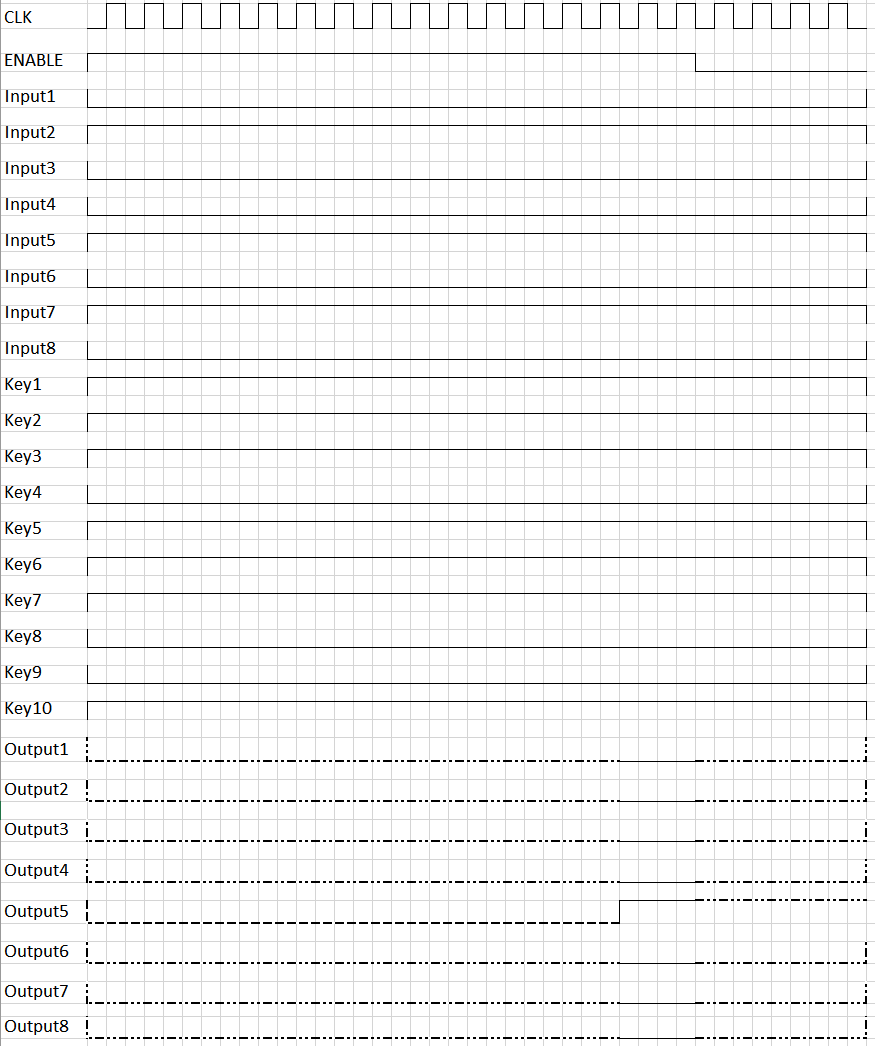
\includegraphics[width=\linewidth]{../img/TimingDiagram_Milestone1.png}
  \caption{Expected Timing Diagram}
  \label{fig:TimingDiagram}
\end{figure}


From our block diagram\ref{fig:BlockDiagram}, we have several stages as explained:

\begin{enumerate}
  \item Key generation to $Shift(P10)$ and $Shift_{3}(P(10))$
  \item Key generation finish
  \item $P(IP)$
  \item $EP(R)$
  \item $EP(R) \oplus key1$
  \item $SBoxes(EP(R) \oplus key1)$
  \item $P4(SBoxes(EP(R) \oplus key1))$
  \item $SW(EP(R) \oplus key1)$
  \item $EP(R)$
  \item $EP(R) \oplus key2$
  \item $SBoxes(EP(R) \oplus key2)$
  \item $P4(SBoxes(EP(R) \oplus key2))$
  \item $IP^{-1}(R,L)$
  \item Put it out on the line.
\end{enumerate}


\begin{figure}
  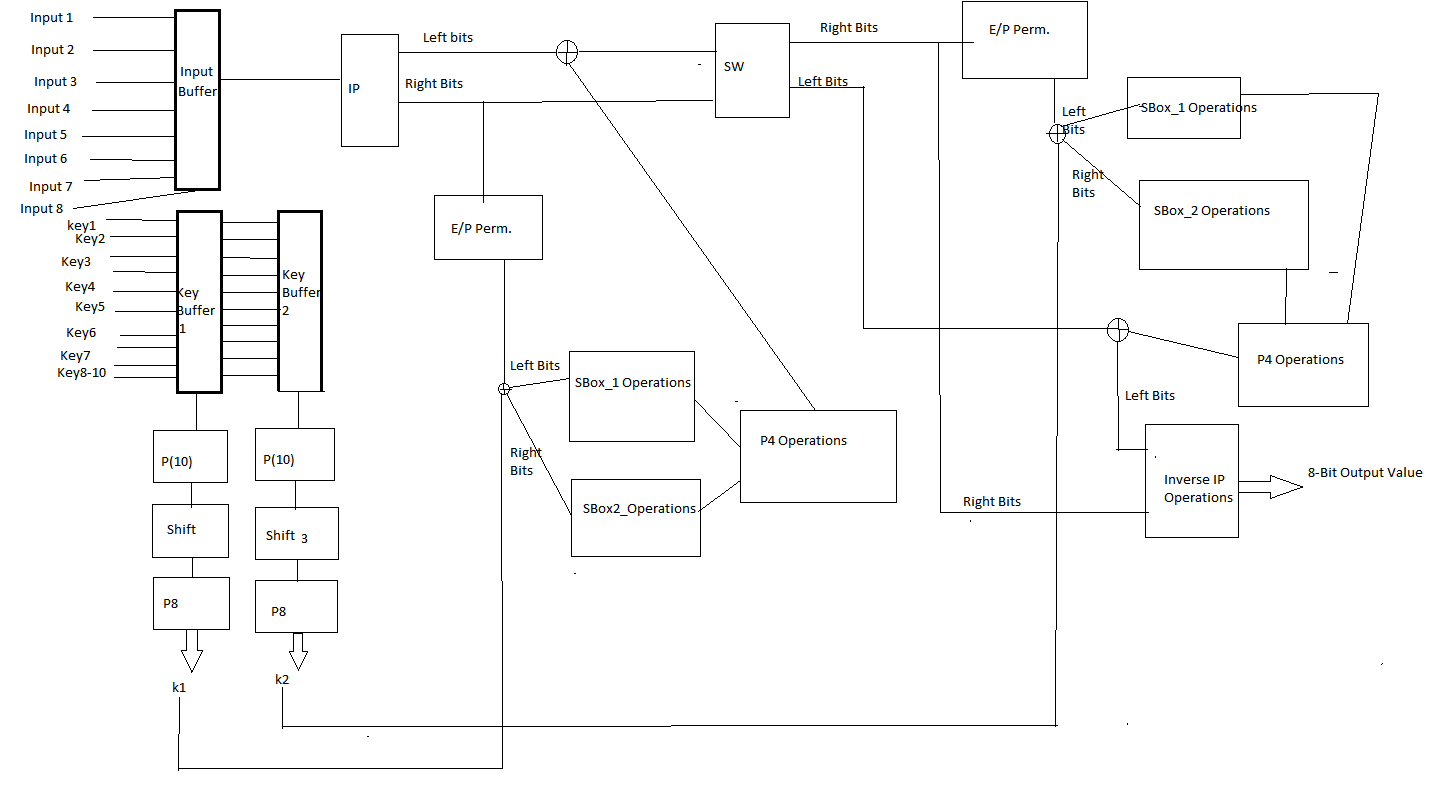
\includegraphics[width=\linewidth]{../img/BlockDiagram_Milestone1.png}
  \caption{Expected Block Diagram}
  \label{fig:BlockDiagram}
\end{figure}
\end{document}
